\documentclass[12pt]{article} % Default font size is 12pt, it can be changed here
\usepackage{geometry} % Required to change the page size to A4
\geometry{a4paper} % Set the page size to be A4 as opposed to the default US Letter
\usepackage{graphicx} % Required for including pictures
\usepackage{float} % Allows putting an [H] in \begin{figure} to specify the exact location of the figure
\usepackage{wrapfig} % Allows in-line images such as the example fish picture
\usepackage{lipsum} % Used for inserting dummy 'Lorem ipsum' text into the template
\usepackage[german]{babel}
\usepackage[ngerman]{datetime}
\usepackage[utf8]{inputenc}
\usepackage{tabularx}
\usepackage{pdflscape}
\usepackage{eurosym}
\usepackage{longtable}
\usepackage{threeparttable}
\usepackage{geometry}
\usepackage[normalem]{ulem}
\usepackage{pdfpages}
\usepackage{listings}
\useunder{\uline}{\ul}{}
\linespread{1.2} % Line spacing

\graphicspath{{img/}} % Specifies the directory where pictures are stored

\begin{document}
\begin{titlepage}

\newcommand{\HRule}{\rule{\linewidth}{0.5mm}} % Defines a new command for the horizontal lines, change thickness here

\center

\textsc{\LARGE TU DRESDEN}\\[1.5cm] % Name of your university/college
\textsc{\Large Service and Cloud Computing}\\[0.5cm] % Major heading such as course name
\textsc{\large Praktikum}\\[0.5cm] % Minor heading such as course title

\HRule \\[0.4cm]
{ \huge \bfseries TimeTracker}\\[0.4cm] % Title of your document

{Eine Microservice-Anwendung für das bessere Zeitmanagement}
\HRule \\[1.5cm]

\begin{minipage}{0.4\textwidth}
\begin{flushleft} 
\emph{Autoren:}\\
Sinthujan \textsc{Thanabalasingam}\\
Wieland \textsc{Strauß}
\end{flushleft}
\end{minipage}
~
\begin{minipage}{0.4\textwidth}
\begin{flushright} 
\emph{Dozentin:} \\
Dr.-Ing. Iris \textsc{Braun} % Supervisor's Name
\end{flushright}

\end{minipage}\\[3cm]

{\large \today}\\[2cm] % Date, change the \today to a set date if you want to be precise

\begin{center}
	
\includegraphics[width=0.5\textwidth]{tu_logo.png}
\end{center}

\vfill % Fill the rest of the page with whitespace

\end{titlepage}

\tableofcontents % Include a table of contents


\begin{figure}[!b]
	\centering
	\includegraphics[scale=1]{logo_TimeTracker.png}
\end{figure}

\newpage % Begins the essay on a new page instead of on the same page as the table of contents 

% Idee, usw. 
\section{Über TimeTracker}

\subsection{Inhalt der Anwendung}
TimeTracker ist eine Anwendung, die es ermöglicht, Zeitinvestitionen zu managen. Ein registrierter Nutzer kann das System nutzen, um den Zeitaufwand bestimmter Aktivitäten aufzuzeichnen. Er kann dazu Activities anlegen und Stoppuhren starten, welche die Dauer der Aufgaben aufzeichnen.

Dem Nutzer wird eine Übersicht über seine aufgenommenen Zeiten angeboten. Dadurch bekommt er einen besseren Überblick darüber, wie viel Zeit er in welche Aufgaben investiert hat. Das Tool soll den Nutzer dabei unterstützen, Hotspots oder Muster in seinem Verhalten zu identifizieren um gegebenenfalls seine Prioritäten anzupassen.

Zusätzlich bietet die Plattform eine anonymisierte globale Statistik, die alle Zeitinvestitionen aller Nutzer repräsentiert und nur von eingeloggten Nutzern eingesehen werden kann.

%Einordnung 
\subsection{Einordnung der Arbeit}
Die Anwendung wurde als Prüfungsvorleistung im Rahmen einer praktischen Übung der Lehrveranstaltung \textit{Service and Cloud Computing} des Lehrstuhls Rechnernetze der TU Dresden entwickelt. Dozentin und Betreuerin ist Frau Dr.-Ing. Iris Braun. 

% Angaben zum Team, Vorgehensweise

\section{Arbeitsablauf}

\subsection{Team}

Das Entwicklerteam besteht aus den Studenten Sinthujan Thanabalasingam  (Master Informatik, 4. Semester) und Wieland Strauß (Diplom Informatik, 7. Semester). 

Sinthujan beschäftigte sich schwerpunktmäßig mit Kozeptionierung und Implementation der Architektur des Backends sowie Entwurf und dem Design des Frontends. Bei Wieland lag der Fokus bei der Implementation im Pair-Programming, der Dokumentation sowie allen organisatorischen Aufgaben.

Die Implementation erfolgte phasenweise im Pair-Programming. Zu Beginn wurde der Fokus auf die benötigte Backend-Funktionalität gelegt, es gab jedoch vorwiegend keine spezifische Aufteilung zwischen Backend- und Frontend-Entwicklung.  

\subsection{Vorgehensweise}

Nach der Ideenfindung wurde zuerst die Architektur entworfen. 
Die Entwicklung wurde nahezu vollständig nach dem Prinzip des Test Driven Development (TDD) betrieben. 
Eine API-Definition wurde zu Beginn mit \textit{Swagger} erstellt und parallel zur Entwicklung des Backends erweitert, wenn neue Anforderungen identifiziert wurden. Da die vorgeschlagene Architektur sich Micro-Services zu nutze macht, wurde bereits während der frühen Entwicklungs- und Testphase Docker als Containertechnik eingesetzt.
Parallel zur Backend-Entwicklung wurde ein auf React basierendes Frontend geschaffen.

Zuletzt wurde die Anwendung auf einem V-Server von DigitalOcean ausgerollt, mit HTTPS abgesichert und unter der Domain \url{https://iamtrent.de} verfügbar gemacht.

Der Arbeitsablauf organisierte sich aus mehreren Treffen. Bei diesen wurde die Planung durchgeführt, ein Großteil der Anwendung geschrieben und Aufgaben für die selbstständige Durchführung festgelegt. Aufgrund der unterschiedlichen Expertise der Entwickler wurde Pair-Programming praktiziert. Weite Teile der Backend-Entwicklung fanden auch nach Absprache bei den Treffen selbstständig, zum Beispiel zu Hause statt.  




%  Verwendete Plattform /Software (Installationshinweise, Versionen)
% Schnittstellenbeschreibung des Web Services (WSDL/WADL/Swagger, …​)
% Umsetzung, Technologien, Sicherheitskonzepte, API

\section{Technologien}


\subsection{Architektur}

%Beschriebender Text?

\begin{figure}[H]
	\hspace{-1.5cm}
	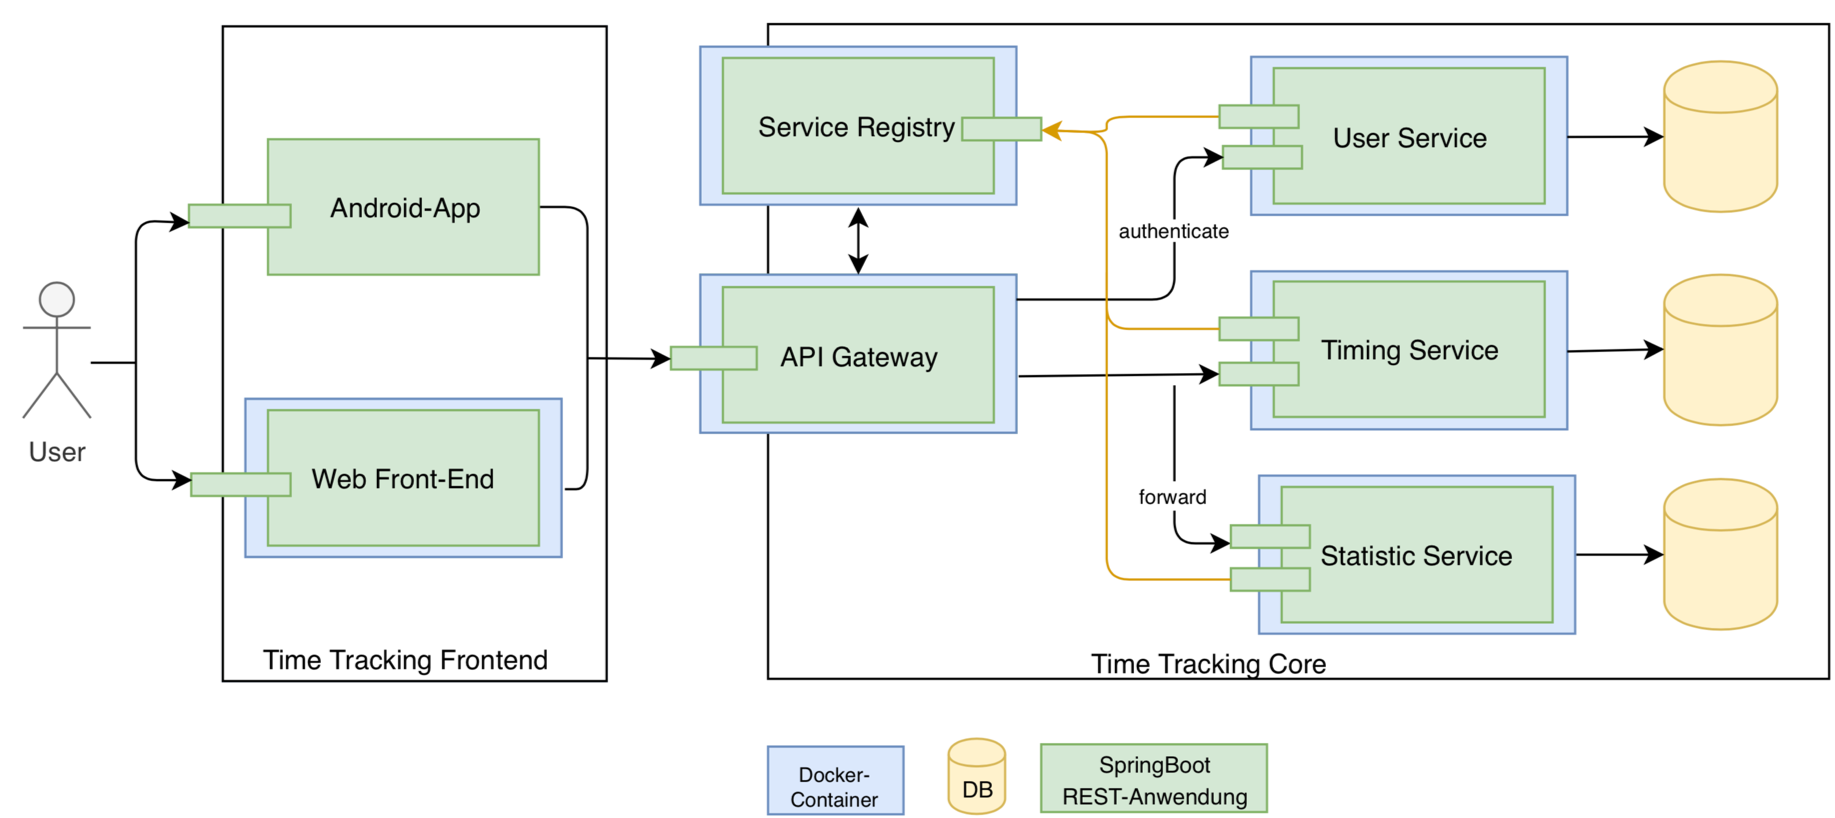
\includegraphics[width=1.15\linewidth]{SCC_Architecture-99final.png}
	\caption{Architektur von TimeTracker}
	\label{fig:Architektur}
\end{figure}

Anmerkung: Die Andoid-App wurde nicht im Rahmen der Lehrveranstaltung fertig gestellt und ist somit noch ausstehend. 

\subsection{Übersicht verwendeter Technologien}
% Tabelle 
\renewcommand{\arraystretch}{1.3} % Für die Abstände zwischen den Spalten 
\begin{table}[H] 
	% \small
	\centering
	\caption{Technologien}
	\begin{tabularx}{\textwidth}{l|c|X}
		\textbf{Name} & \textbf{Version} & \textbf{Verwendung} \\
		\hline
		Java & JDK 1.8.0 & Verwendete Programmiersprache \\
		Mavent & 3.1.0  & Build-Management-Tool \\
		Spring boot & 2.0.2 & Java Framework für Web-Systeme \\
		MySQL & 5.7.0 & Relationale Datenbank \\
		Netflix Zuul & 1.3.1 & Edge Service für dynamisches Routen, \newline Monitoring und Sicherheit  \\
		Netflix Eureka & 1.9.2 & REST-basierter Service,  Zuordnen von Services   \\
		JSON & - & Dateiformat bei Übermittlung \\
		REST & - & Programmierparadigma für Webservices \\
		React & 16.1.1 & JavaScript Bibliothek für User Interfaces  \\
		single-spa & 2.6.0 & JavaScript Framework für Front-End Microservices \\
		OpenAPI  (Swagger) & 3.0. & REST-Schnittstelle basiert auf Standard von OpenAPI,  Zum Entwerfen und Dokumentieren der RESTfull-Schnittellen wurde das Framework Swagger verwendet \\
		Postman & 6.5.3 & API Development Environment \\
		Docker & 18.09.0 & Umgebung für Container \\
	\end{tabularx}
	\label{tab:Technologien}
\end{table}

\subsection{Schnittstellenbeschreibung}
% Links von Server mit http://editor.swagger.io/ oder https://swagger.io/tools/swagger-inspector/ or https://swagger.io/tools/swagger-ui/

Die API wurde nach dem OpenAPI-Standard entwickelt und generierte automatisch ein Controller in Java. Eine Auflistung aller Methoden ist über die folgenden Links zu erreichen. Zusätzlich befindet sich im Anhang (Seite \pageref{Anhang}) ein Ausdruck der automatisch generierten Dokumentation.

\begin{itemize}
	\item frontend-service: 
	\item timing-service: 
	\item user-service:
\end{itemize}

\subsection{Sicherheit}

Die Sicherheit wurde mittels \textbf{JSON Web Token (JWT)} und umgesetzt. Dabei erhält der Benutzer beim Login eine UUID, mittels derer er sich gegenüber den Diensten authentifizieren kann. 

Des weiteren wird die Sicherheit der Verbindung mittels der Transportverschlüsselung \textbf{HTTPS} gewährleistet. 


% Bedienungsanleitung für Clients

%\epigraph{	Your Time is precius. \newline Track your investments!}{\textit{Group 4}} %Raus mit dem kleinen Scherz??
\section{Bedienungsanleitung des Clients}
% So schön mit Bildern und so, erst bei fertiger Anwendung 

\begin{center}
	\textit{Your Time is precius. \newline Track your investments!}
\end{center}


TimeTracker bietet folgende Funktionen:
\begin{itemize}
	\item Time Tracking
	\item Anlegen und Löschen von Aktivitäten % durch User
	\item Tracking für verschiedene Aktivitäten
	\item Zuordnen mit Tags
	\item Abruf von Statistiken (Benutzer/Global)
\end{itemize}


Der Dienst ist online zu erreichen unter \url{https://iamtrent.de}

Lokale Installationen sind zu erreichen unter localhost:9123

\subsection{Build}

Zum Bild bitte folgende Zeilen Ausführen:
\begin{lstlisting}[language=bash]
	mvn clean install
	docker-compose -f docker/docker-compose.yml up -d
\end{lstlisting}

\subsection{Registrieren und Login }
 
 \begin{figure}[H]
 	\hspace{-1.5cm}
 	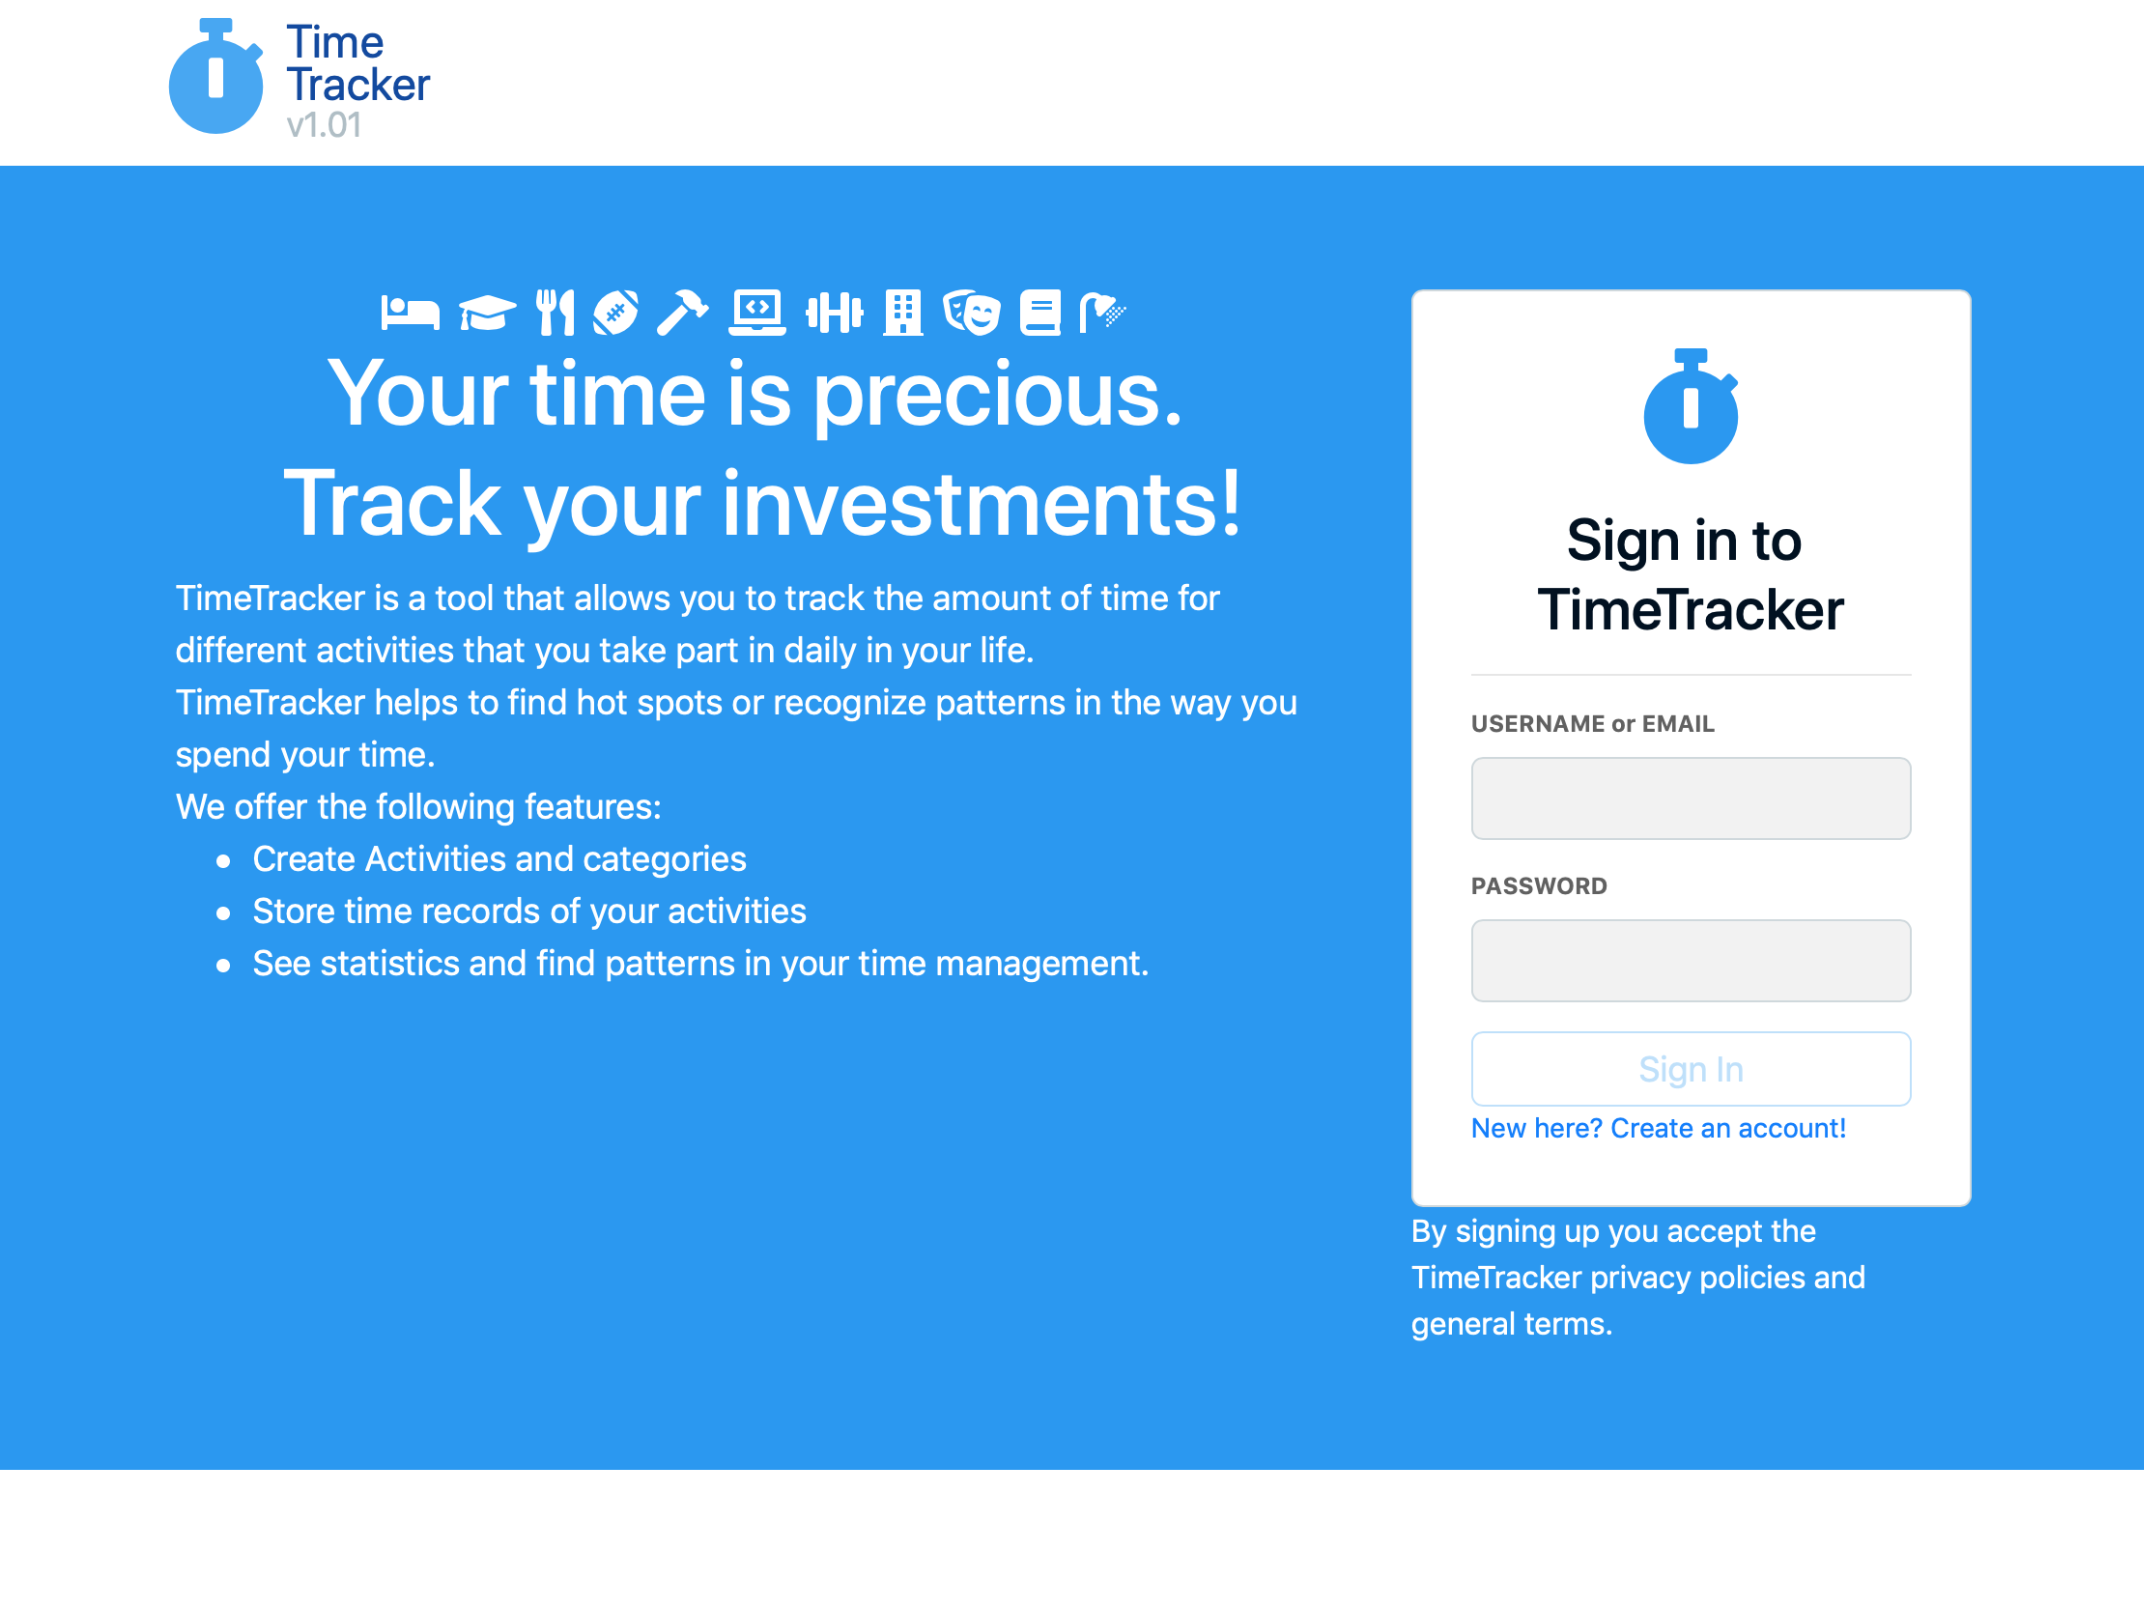
\includegraphics[width=1.15\linewidth]{login.png}
 	\caption{Login}
 	\label{fig:login}
 \end{figure}

Willkommen bei TimeTracker! Auf unserer Startseite (Abb. \ref{fig:login}) kannst du dich mit deinen Benutzerdaten einloggen.  
Du hast noch kein Benutzerkonto? Kein Problem, unterhalb des \textit{Sign In} Buttons ist ein Link, der zur Registrierung führt.
 

\begin{figure}[H]
	\hspace{-1.5cm}
	\centering
	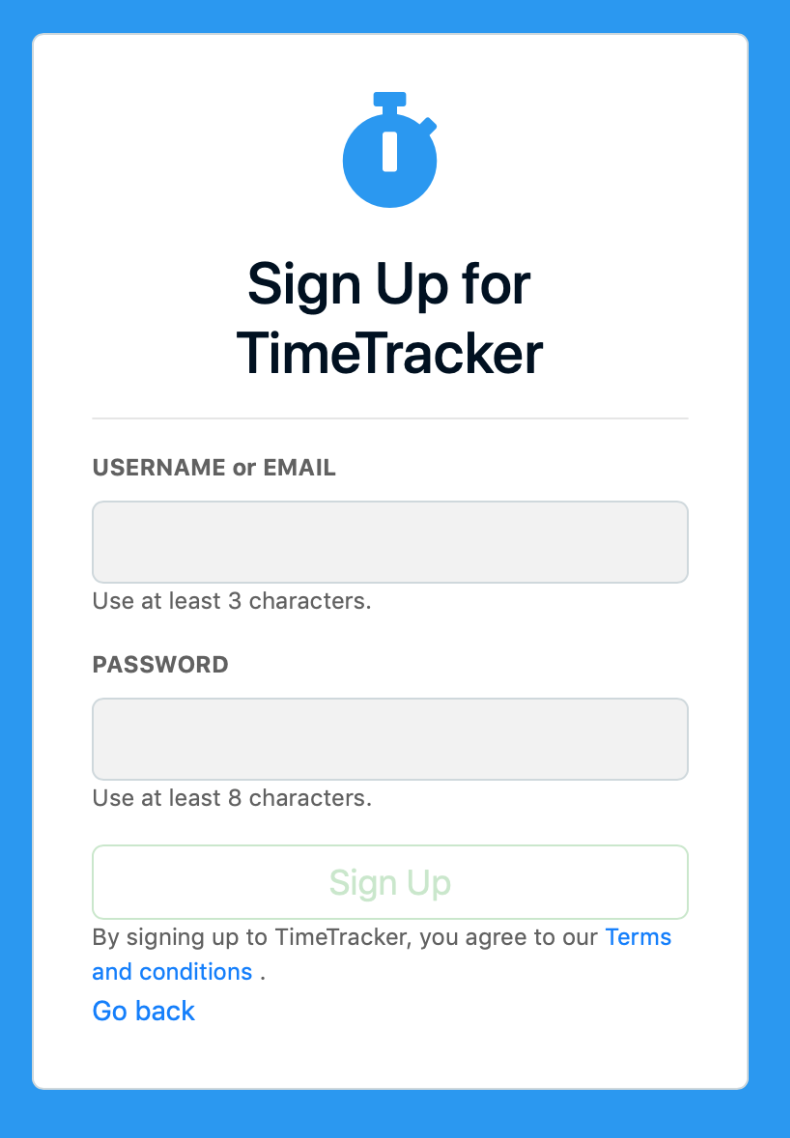
\includegraphics[scale=0.5]{register.png}
	\caption{Registrieren}
	\label{fig:register}
\end{figure}
%\newpage
%\begin{wrapfigure}{l}{0.5\textwidth}
%		\hspace{-1.5cm}
%		\centering
%		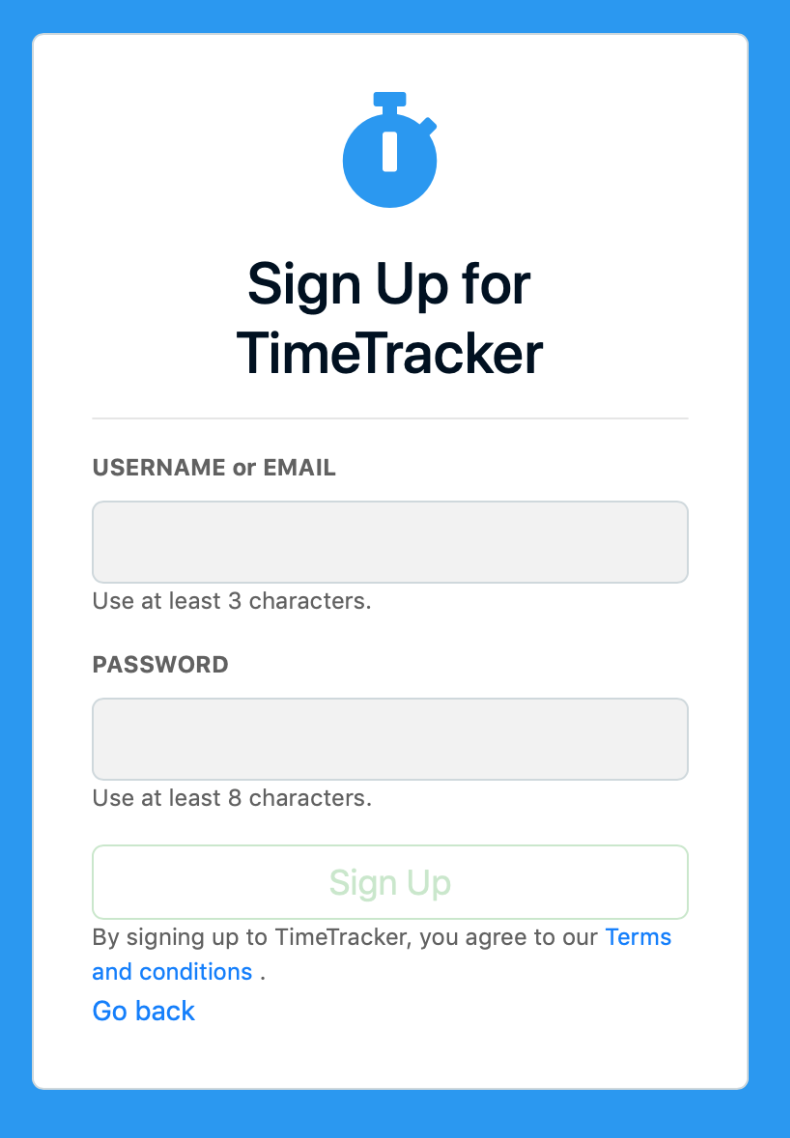
\includegraphics[width=0.38\textwidth]{register.png}
%		\caption{Registrieren}
%		\label{fig:register}
%\end{wrapfigure}

Um die zu registrieren musst du nur einen Usernamen oder eine Email, sowie ein Passwort eintragen. Beachte, dass das Passwort mindestens 8 Zeichen haben muss, vorher ist der Button nicht anklickbar! 
Nach dem du dich erfolgreich registriert hast wirst du wieder auf unsere Startseite (Abb. \ref{fig:login}) geleitet, wo du dich ab sofort mit deinen Nutzerdaten anmelden kannst. 

Wenn du einmal angemeldet bist kannst du dich jeder Zeit mit einem Klick auf \textit{Logout} oben rechts wieder abmelden.

\subsection{TimeTracken}

Wenn du dich das erste mal einloggst, sind noch keine Aktivitäten vorhanden. 
Aktivitäten sind die Aktionen, für die du deine Zeit trackst. 
Füge einfach eine neue Aktivität hinzu, in dem du auf \textit{+ New Aktivity} klickst (Abb. \ref{fig:no_activity}). 

\begin{figure}[H]
	\hspace{-1.5cm}
	\centering
	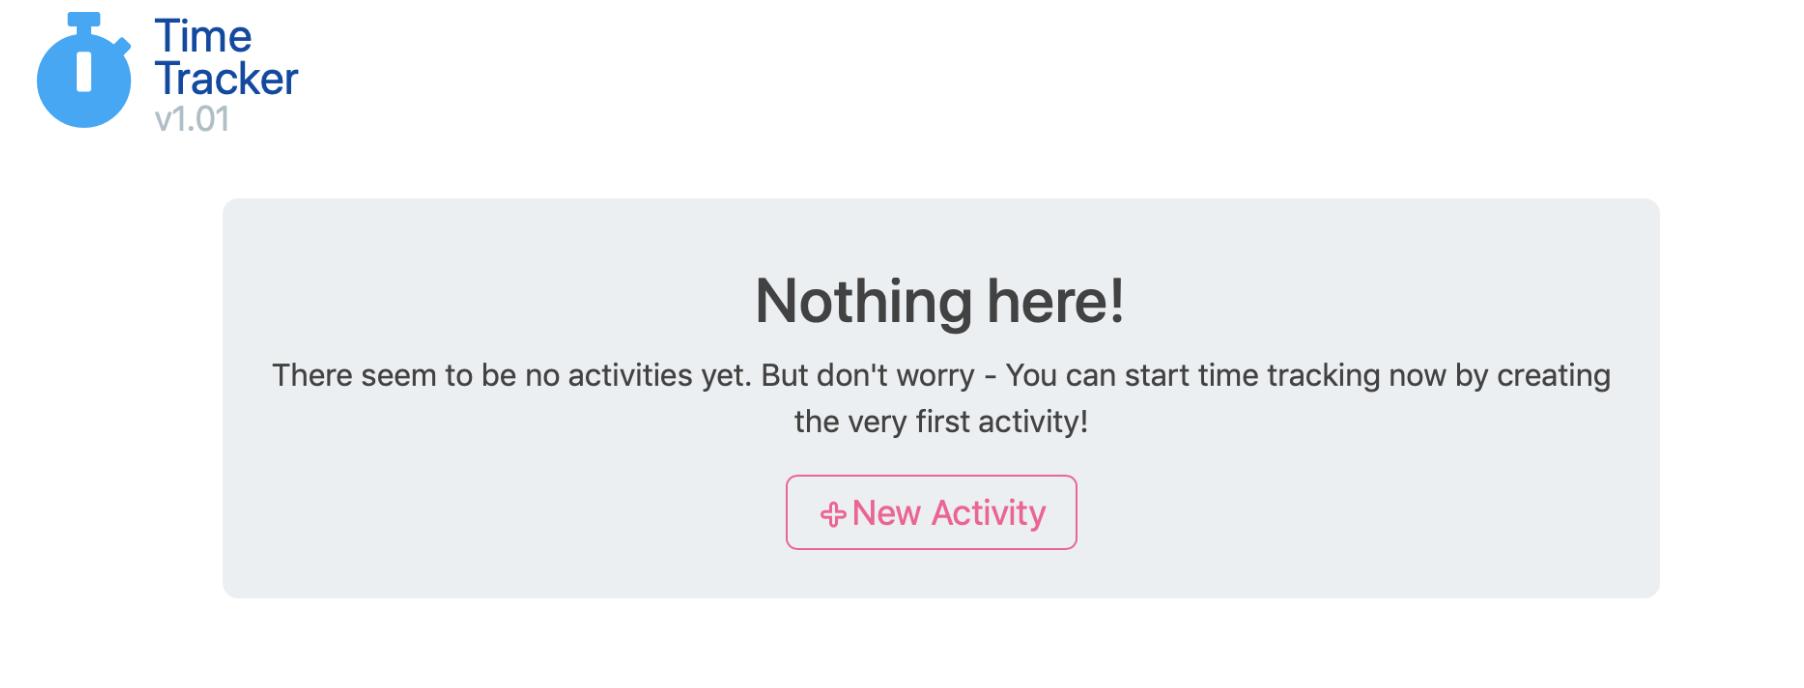
\includegraphics[scale=0.5]{no_activity.png}
	\caption{Keine Aktivitäten angelegt}
	\label{fig:no_activity}
\end{figure}

\begin{figure}[H]
	\hspace{-1.5cm}
	\centering
	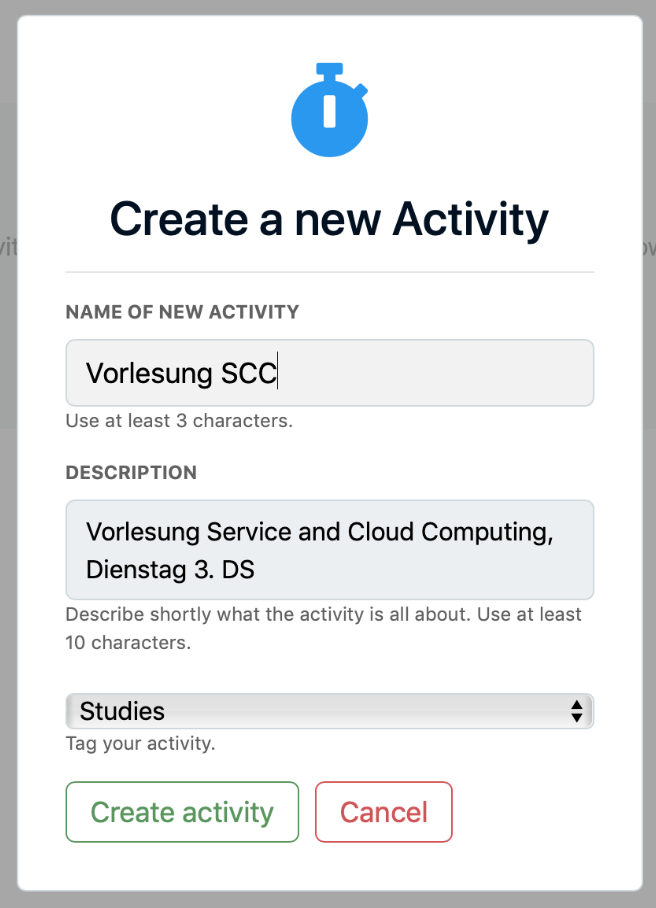
\includegraphics[scale=0.5]{create_activity.png}
	\caption{Aktivität anlegen}
	\label{fig:create_activity}
\end{figure}

Nun kannst du eine Aktivität anlegen (Abb. \ref{fig:create_activity}. 
Gibt ihr einen Namen und eine Beschreibung, damit du später weißt, wofür du sie angelegt hast. 
Der Name darf keine Umlaute wie \glqq Ä, Ö, Ü\grqq{}  enthalten und die Beschreibung muss mindeste 10 Zeichen lang sein. 
Danach verbindest du deine Aktivität mit einem Tag. Tags sind sowas wie Kategorien. 
Jede Aktivität hat ein Tag und dadurch eine Zuordnung zu einem deiner Lebensbereiche. 

Tags sind beispielsweise Studies, Sport und Relax. 
Mit Hilfe der Tags kannst du später schauen, wie viel Sport du gemacht hast, auch wenn du deine Zeit in den Aktivitäten "Schwimmen" und "Rad fahren" aufgenommen hast. 


\begin{figure}[H]
	\hspace{-1.5cm}
	\centering
	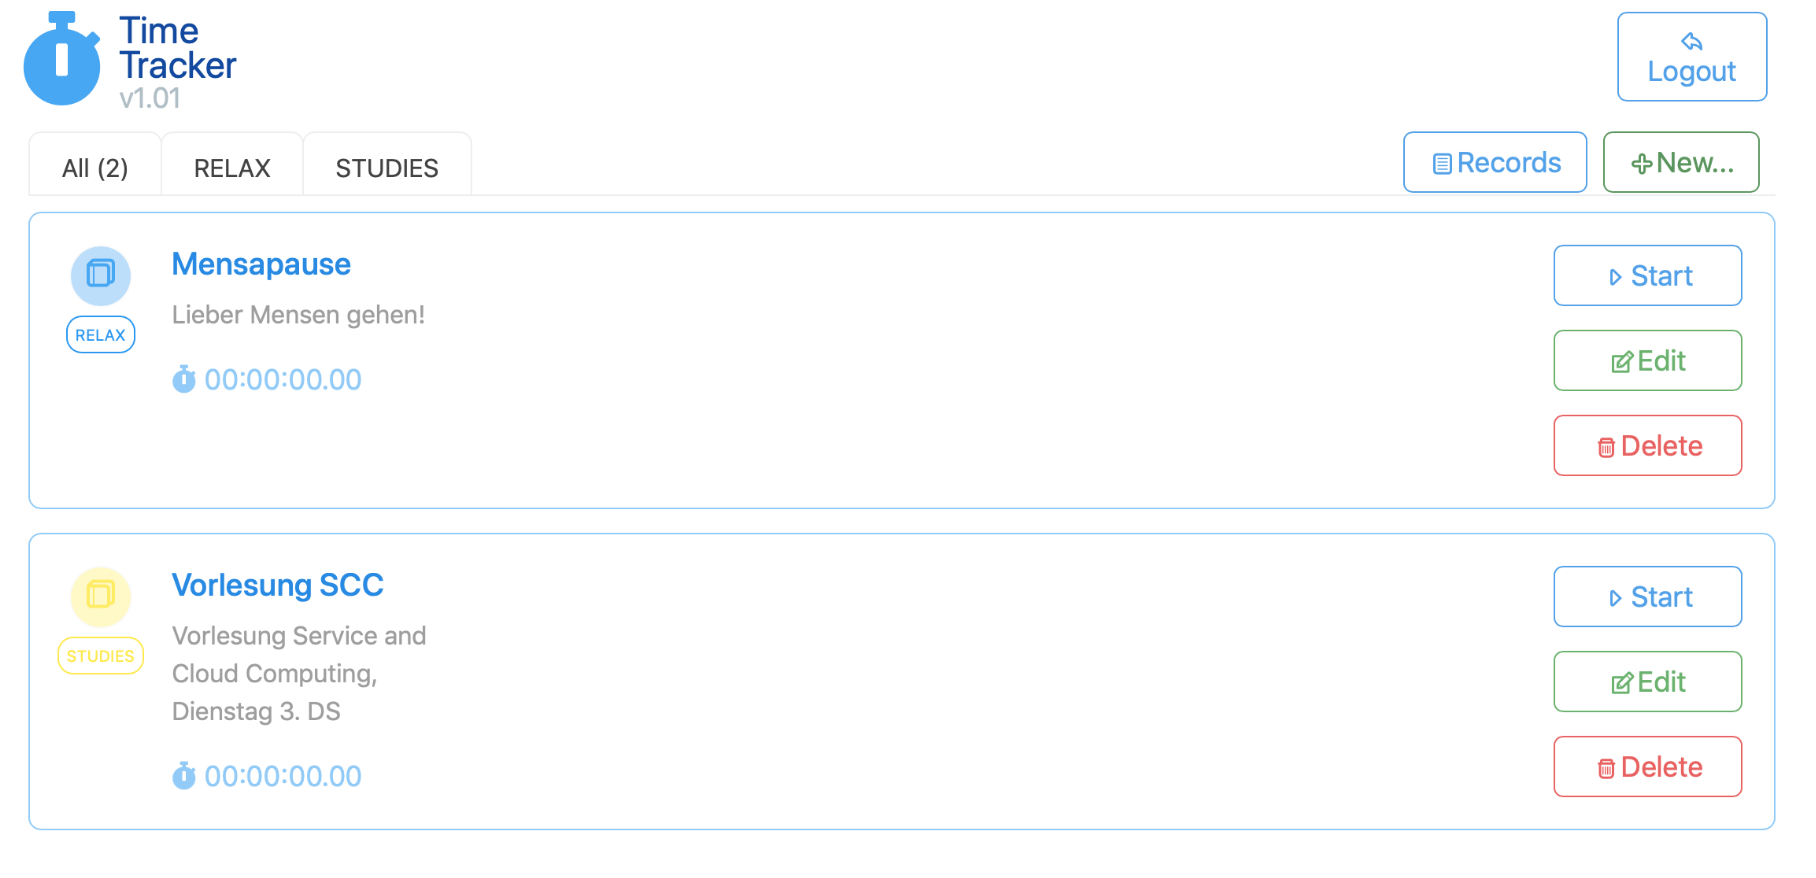
\includegraphics[scale=0.5]{activitys.png}
	\caption{Übersicht: Aktivitäten}
	\label{fig:activitys}
\end{figure}

Nun hast du Aktivitäten und eine Übersicht (Abb. \ref{fig:activitys}. Hier kannst du mit einem Klick auf  \textit{Start}  ein Record beginnen. Records sind die einzelnen Aufnahmen, die du machst. Zusammen addiert ergeben sie die gesamte Zeit, die du für eine Aktivität aufbringst. Wie du siehst, blinkt nun die Uhr und die Zeit läuft. 
Mit einem Klick auf den selben Button stoppst du das Tracking deiner Aktivität und beendest den Record. Die Zeit des Records wird dir nun angezeigt.
 Du kannst dich zwischendurch auch abmelden oder von einem anderen Gerät aus einloggen, die Aufnahme geht einfach weiter. 

Mit dem Button \textit{+ New} kannst du weitere Aktivitäten anlegen und mit dem Button \textit{Delete} die jeweilige auch wieder löschen. In dem du auf \textit{Edit} klickst kannst du die Inhalte updaten. 

Über die Reiter oben kannst du deine Aktivität nach den von dir genutzten Tags filtern. 

\begin{figure}[H]
	\hspace{-1.5cm}
	\centering
	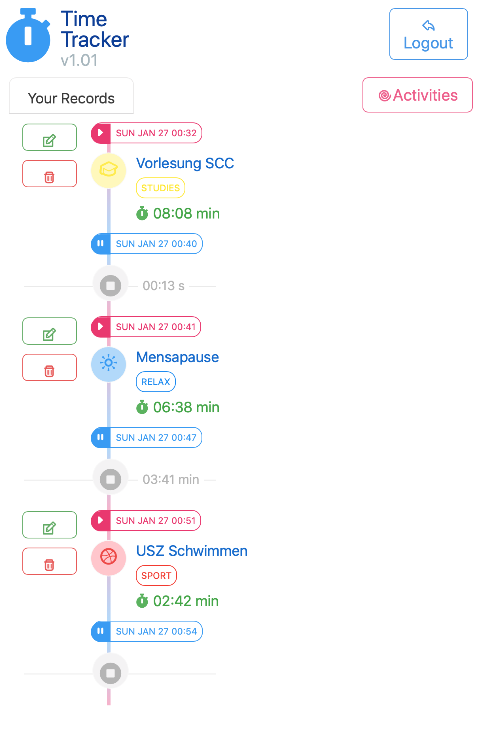
\includegraphics[scale=0.5]{records_new.png}
	\caption{Aufgenommene Records}
	\label{fig:records}
\end{figure}

Wenn du \textit{Records} anwählst kommst du zu einer Übersicht all deiner Zeitaufnahmen (Abb. \ref{fig:records}). Hier steht für welche Aktivität und Tag, von wann bis wann und wie lange die Aufnahmen war. Ebenso kannst du Records löschen. 


% Feedback + Kritik am Praktikum

\section{Feedback und Kritik am Praktikum}

\paragraph{Allgemein:} Insgesamt machte es viel Spaß, diese Anwendung zu entwickeln. Ein gutes Klima im Team trug maßgeblich dazu bei. 
Aufgrund des unterschiedlicher praktischer Erfahrung fand ein reger Wissensaustausch statt. Es entwickelte sich mit der Zeit eine Art Mentoring zwischen beiden Teilnehmern.
Bei der Umsetzung wurde sehr deutlich, wie das Praktikum die Vorlesungsinhalte vertieft und in direkten praktischen Bezug dazu tritt. Das in der Vorlesung erlangte Wissen konnte anschaulich umgesetzt werden. Die im Rahmen des Praktikums entstandene Anwendung wird weiterentwickelt und genutzt werden.


\paragraph{Spezifikation der Anforderungen:} Durch die in manchen Teilen unspezifische Aufgabenstellung ließ sich schwer abschätzen, welche Anforderungen genau erfüllt werden müssen.
Positiv daran ist die Möglichkeit der freien Auswahl von Vorgehensweise, Umsetzung und Tools.
Die Zwischenpräsentation und das Feedback darauf hat jedoch maßgeblich zum besseren Verständnis der Aufgabenstellung und fokussierterem Arbeiten geführt.

\section{Anhang}
\begin{itemize}
	\item Generierte API-Dokumentation User Service 
	\item Generierte API-Dokumentation Timing Service 
	\item Generierte API-Dokumentation Frontend Service 
\end{itemize}
\label{Anhang}

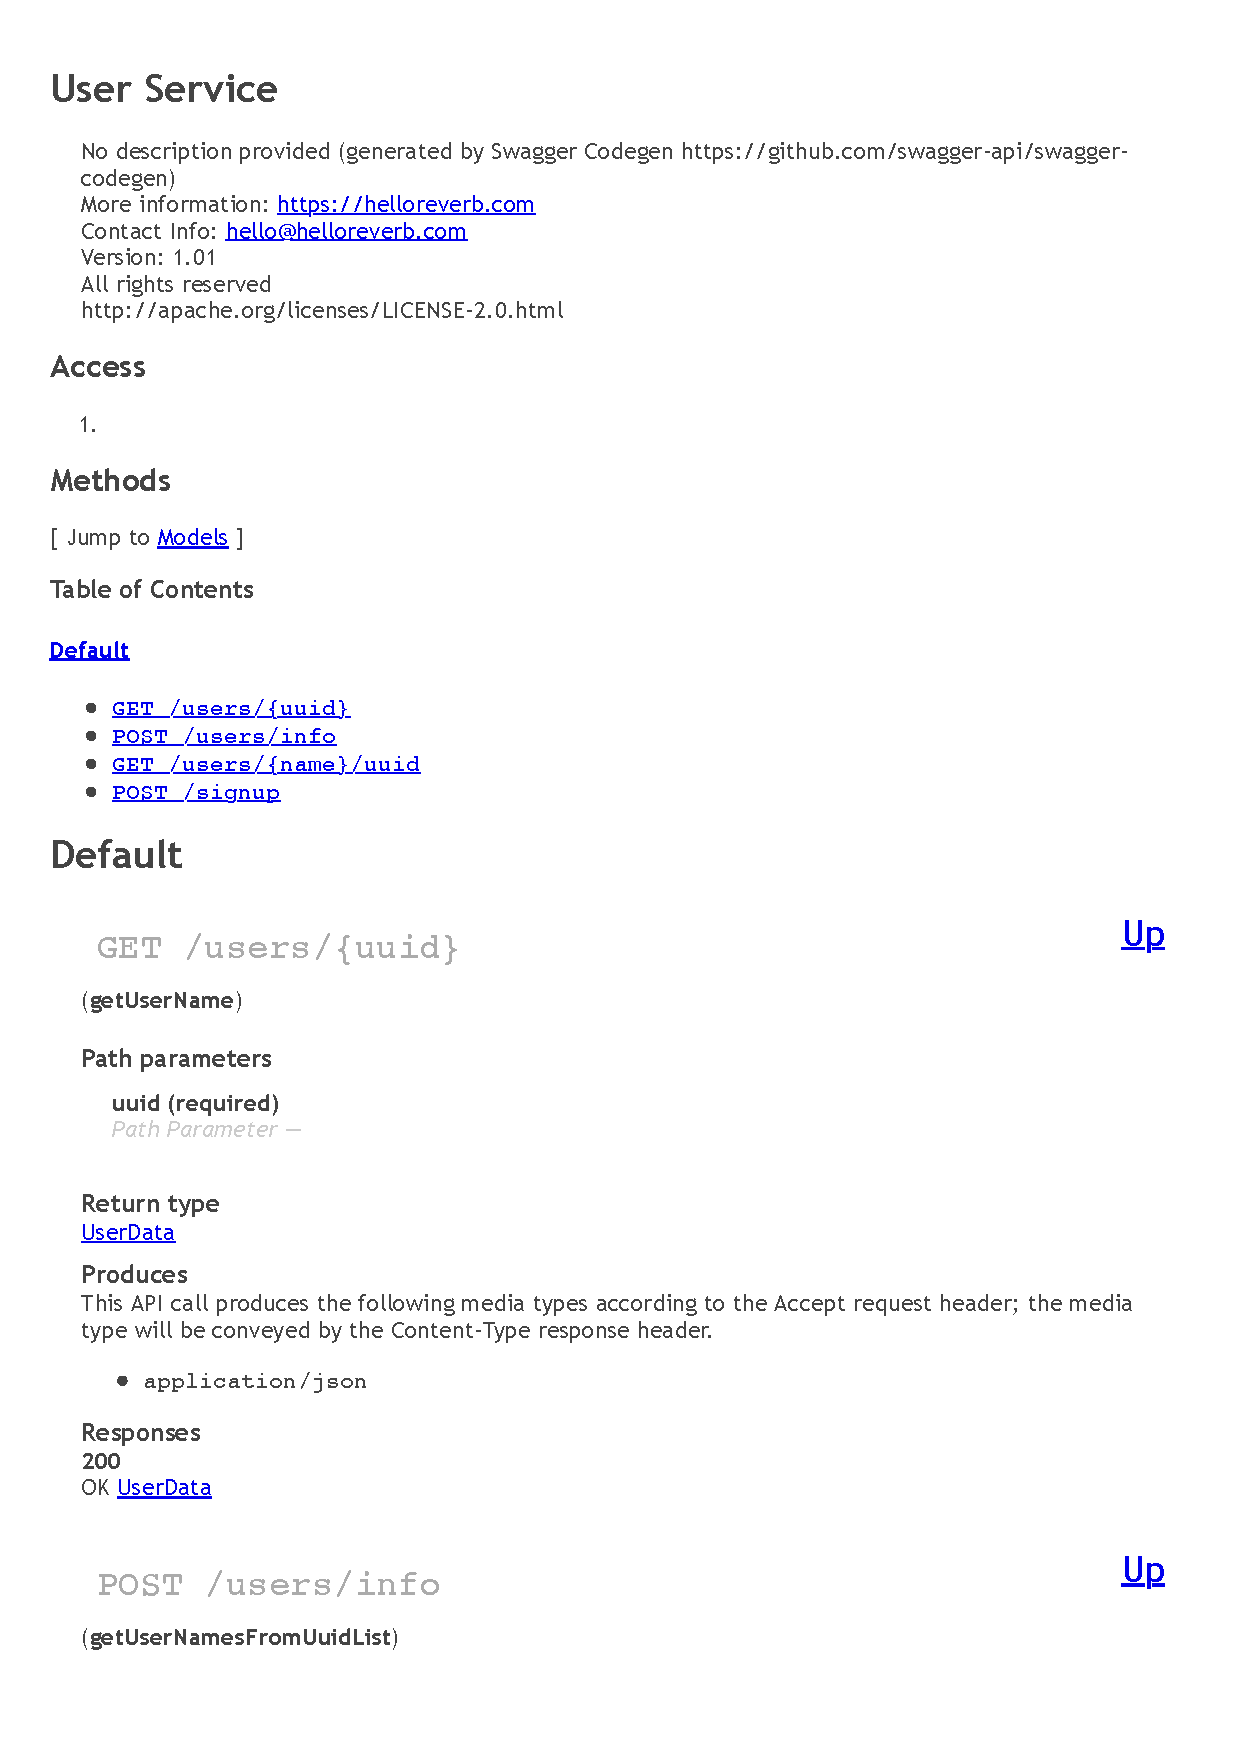
\includepdf[pages=-]{Anhang/User_Service}
\label{pdf:UserService}

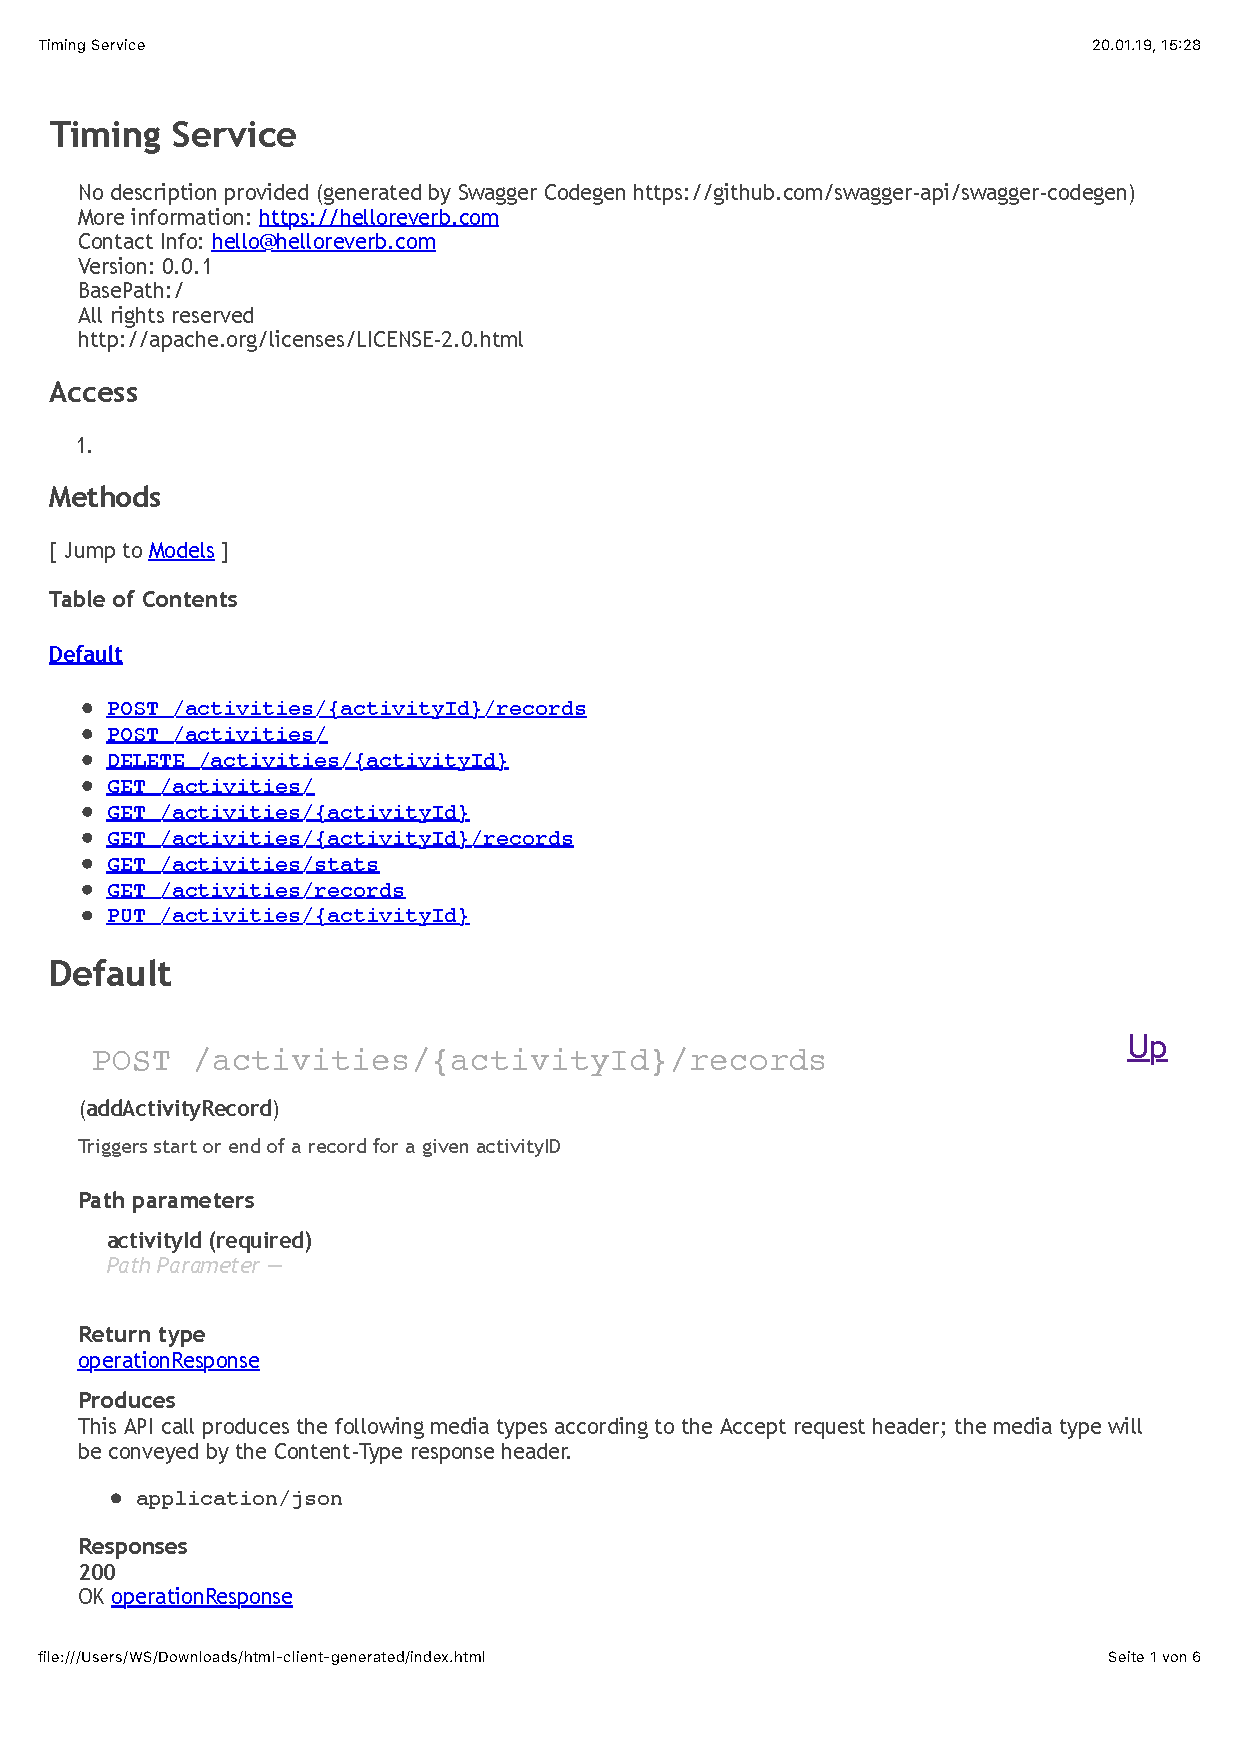
\includepdf[pages=-]{Anhang/Timing_Service}
\label{pdf:TimingService}


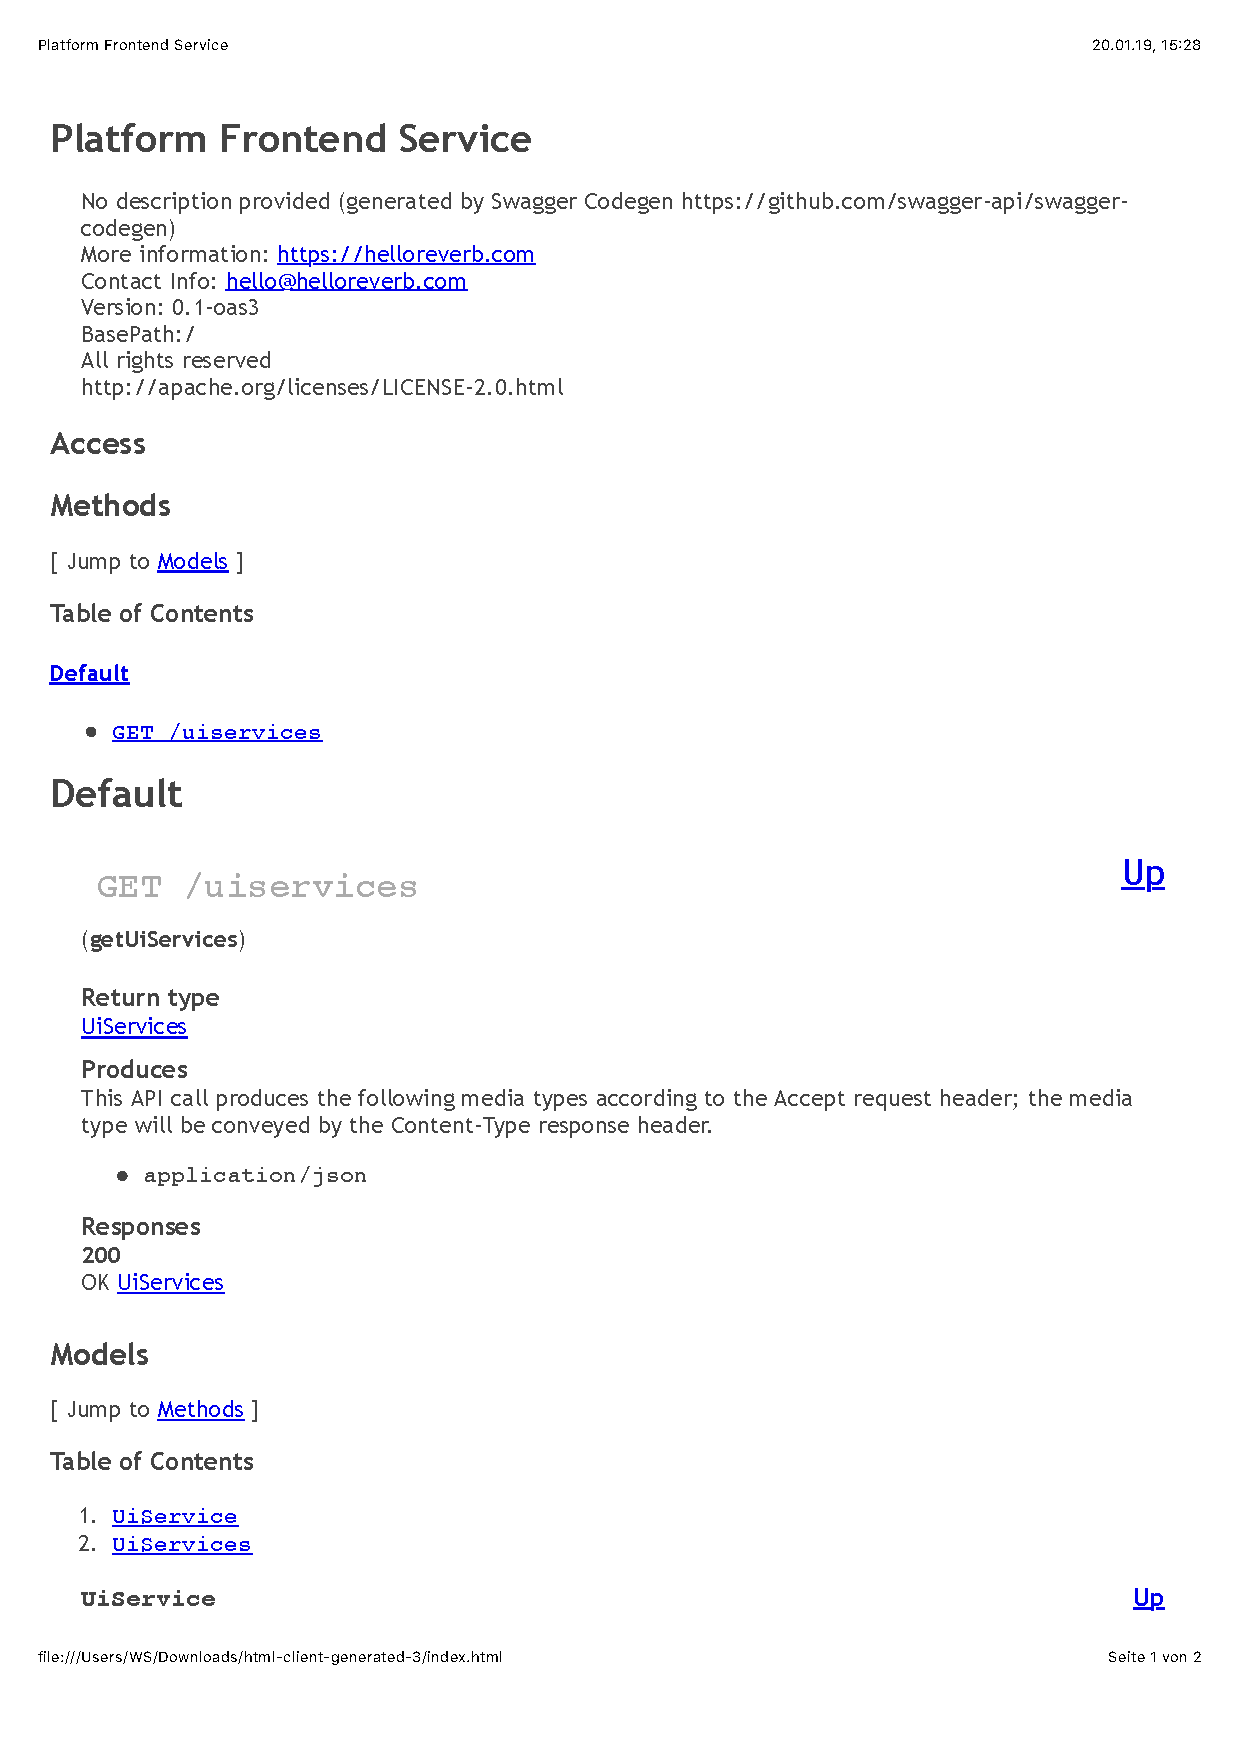
\includepdf[pages=-]{Anhang/Frontend_Service}
\label{pdf:FrontendService}

\end{document}
